\section{Consumption, saving and investment}

\subsection{Consumption and saving}

The aggregate level of desired consumption, $C^d$ is the sum of of the desired consumption of all households. The desired national saving, $S^d$ is the level of national saving that occurs when aggregate consumption is at $C^d$. In a closed economy, 
\[
    S^d = Y - C^d - G
\]

\subsubsection{Inter-temporal Consumption Model}


\begin{definition}
    An individual's \textbf{Present Value of Lifetime Resources, $PVLR$} is defined as 
    \[
        PVLR = a + y + \frac{y^f}{1 + r}
    \]
    Where 
    \begin{align*}
        a &= \text{assets, current period} \\ 
        y &= \text{income, current period} \\ 
        y^f &= \text{future income, current period}
    \end{align*}
\end{definition}

\begin{definition}
    An individual's \textbf{Present Value of Lifetime Consumption, $PVLC$} is defined as 
    \[
        PVLC = c + \frac{c^f}{1 + r}
    \]
    Where 
    \begin{align*}
        c &= \text{consumption, current period} \\ 
        y &= \text{consumption, future period}
    \end{align*}
    
\end{definition}



\begin{definition}
    An individual's \textbf{budget constraint} is given by
    \begin{align*}
        PVLC &= PVLR \\
        c + \frac{c^f}{1 + r} &= (a + y) + \frac{y^f}{1+r} \\
        c^f &= (a + y - c) (1 + r) + y^f \\
        &= \underbrace{(a + y)(1 + r)+ y^f}_{intercept}   \underbrace{ - (1+r)}_{slope} c 
    \end{align*}

\end{definition}
\begin{center}
    \begin{tikzpicture}
    % ---- editable parameters ----
    \pgfmathsetmacro{\r}{0.25}   % interest rate r
    \pgfmathsetmacro{\yf}{4}     % y^f (future endowment)
    \pgfmathsetmacro{\ay}{4}     % a + y (current resources)
    \pgfmathsetmacro{\slope}{-(1+\r)}           % slope = -(1+r)
    \pgfmathsetmacro{\xPVLR}{\ay - (\yf / \slope)}% x-intercept (PVLR point)
    \pgfmathsetmacro{\yintercept}{\ay * (1 + \r) +\yf}% y-intercept
    % -----------------------------

    \begin{axis}[
    xmin=0, xmax=10,
    ymin=0, ymax=10,
    axis lines* = left,
    xtick={0}, ytick=\empty,
    clip=false,
    scale=0.9,
    ]
    % Budget line: c^f = y^f + slope*(c - (a+y))
    \addplot[domain=0:10, restrict y to domain=0:10, samples=400, color=blue, very thick]
        {(\yf + \ay * (1 + \r)) + \slope * x};

    % Guides from F to axes
    \addplot[color=black, thick, dashed] coordinates {(0,\yf) (\ay,\yf)};
    \addplot[color=black, thick, dashed] coordinates {(\ay,0) (\ay,\yf)};

    % Point F (no-borrowing, no-lending)
    \addplot[color=teal, mark=*, only marks, mark size=3pt] coordinates {(\ay,\yf)};
    \node[above right] at (\ay,\yf) {$F$};

    % Axis labels
    \node[right] at (current axis.right of origin) {Current consumption, $c$};
    \node[above] at (current axis.above origin) {Future consumption, $c^f$};

    % Intercept labels
    \node[left]  at (0,\yf) {$y^{f}$};
    \node[below] at (\ay,0) {$a{+}y$};

    % Slope annotation
    \node[align=left] at (6.2,8.1) {Slope $=-(1+r)$};
    \draw[-Triangle] (5.8,7.7) to [out=210, in=45] (4.0,6.8);

    % No-borrowing/no-lending label
    \node[align=left, right] at (6.5,3) {No-borrowing,\\no-lending point};
    \draw[-Triangle] (6,3) -- (\ay+0.1,\yf);

    % Vertical intercept label 
    \node[align = left, left] at (0, \yintercept) {$y^f + (a + y) ( 1 + r)$};

    % PVLR at x-intercept
    \node[below] at (\xPVLR,0) {\textit{PVLR}};
    \end{axis}
    \end{tikzpicture}
\end{center}

\begin{remark}
    We can classify individuals as lending or borrowing 
    \begin{itemize}
        \item lending, if $c < a + y \iff a + y - c > 0$
        \item borrowing if $c > a + y \iff a + y - c < 0$
    \end{itemize} 
\end{remark}


\begin{remark}
    We can classify individuals as saving or dissaving
    \begin{itemize}
        \item saving, if $y > c$
        \item dissaving, if $y < c$
        \begin{itemize}
            \item borrowing, if $c > y + a \iff a + y - c < 0$
        \end{itemize} 
    \end{itemize} 

    \textbf{Dissaving} $\neq$ \textbf{Borrowing}.
\end{remark}

\begin{remark}

In choosing between $c$ and $c^f$, consumers face diminishing marginal utility. The indifference curve has the shape

\begin{center}
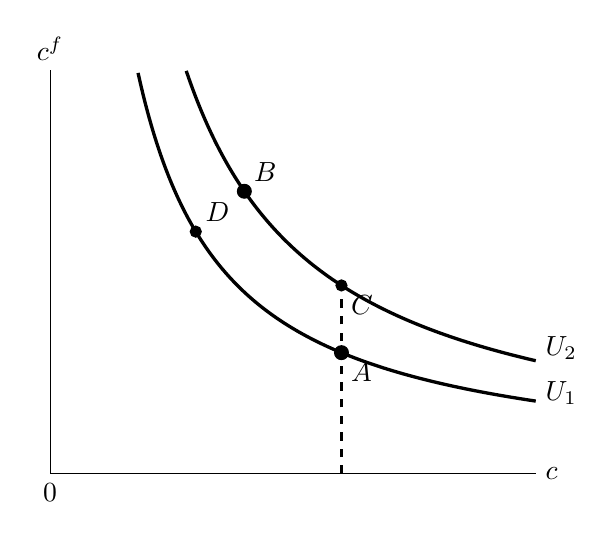
\begin{tikzpicture}
% --- choose convenient "hyperbola" ICs: c^f = k / c ---
\pgfmathsetmacro{\kone}{18}   % level U1 (lower IC)
\pgfmathsetmacro{\ktwo}{28}   % level U2 (higher IC)
\pgfmathsetmacro{\cA}{6.0}    % c-coordinate of A and the dashed line
\pgfmathsetmacro{\cfA}{\kone/\cA}
\pgfmathsetmacro{\cfOnUtwoAtcA}{\ktwo/\cA} % comparison point on U2 at same c
\pgfmathsetmacro{\cB}{4.0}
\pgfmathsetmacro{\cfB}{\ktwo/\cB}

\pgfmathsetmacro{\dx}{\cB-1}
\pgfmathsetmacro{\dy}{\kone/(\cB-1)}

\begin{axis}[
  xmin=0, xmax=10,
  ymin=0, ymax=10,
  axis lines* = left,
  xtick={0}, ytick=\empty,
  clip=false,
  scale=0.9,
]
  % Indifference curves
  \addplot[
    domain=1:10, restrict y to domain=0:10,
    samples=400, color=black, very thick
  ] {\kone/x};
  \addplot[
    domain=1:10, restrict y to domain=0:10,
    samples=400, color=black, very thick
  ] {\ktwo/x};

  % Points A (on U1) and B (on U2)
  \addplot[color=black, mark=*, only marks, mark size=2.5pt] coordinates {(\cA,\cfA)};
  \node[below right] at (\cA,\cfA) {$A$};
  \node[below right] at (\cA,\cfOnUtwoAtcA) {$C$};

  \addplot[color=black, mark=*, only marks, mark size=2.5pt] coordinates {(\cB,\cfB)};
  \node[above right] at (\cB,\cfB) {$B$};
  \node[above right] at (\dx,\dy) {$D$};
  \addplot[color=black, mark=*, only marks, mark size = 2pt] coordinates {(\dx,\dy)};

  % Vertical dashed line at c = c_A and the comparison point on U2
  \addplot[color=black, dashed, thick] coordinates {(\cA,0) (\cA,\cfOnUtwoAtcA)};
  \addplot[color=black, mark=*, only marks, mark size=2pt] coordinates {(\cA,\cfOnUtwoAtcA)};

  % Axis labels
  \node[right] at (current axis.right of origin) {$c$};
  \node[above] at (current axis.above origin) {$c^{f}$};

  % Curve labels
  \node[right] at (10,\kone/9) {$U_1$};
  \node[right] at (10,\ktwo/9) {$U_2$};

\end{axis}
\end{tikzpicture}
\end{center}

To convince ourselves that $B$ is preferred to $A$
\begin{itemize}
    \item $C$ has more $c^f$ than $A$ and the same $c$, hence
    \[
        A \prec C \sim B
    \]
    \item $A$ is equally desireable as $D$, which has less $c$ and $c^f$  than $B$
    \[
        A \sim D \prec B
    \]
\end{itemize} 
\end{remark}

\begin{remark}
    Optimal consumption is the point of tangency of the budget constraint and the indifference curve.

\begin{center}
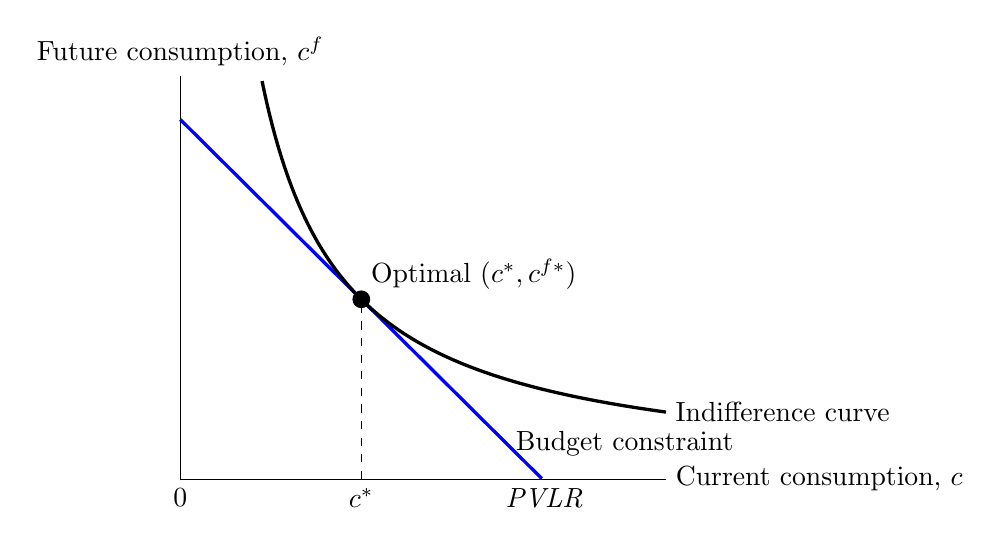
\begin{tikzpicture}
% ====== EDIT THESE ======
\pgfmathsetmacro{\r}{0.25}   % interest rate r
\pgfmathsetmacro{\ay}{5.0}   % present resources a + y
\pgfmathsetmacro{\yf}{4.0}   % future endowment y^f
% ========================

% --- Derived quantities (do not edit) ---
\pgfmathsetmacro{\slope}{-(1+\r)}                % budget slope = -(1+r)
\pgfmathsetmacro{\PVLR}{\ay + \yf/(1+\r)}        % x-intercept (PVLR)
\pgfmathsetmacro{\Yint}{(1+\r)*\ay + \yf}        % y-intercept
% Tangency with IC c^f = k/c:  -k/c^2 = -(1+r) => k=(1+r)c^{*2};  also c^f*=(1+r)c* on BL
\pgfmathsetmacro{\cstar}{(\yf + (1+\r)*\ay)/(2*(1+\r))}
\pgfmathsetmacro{\cfstar}{(1+\r)*\cstar}
\pgfmathsetmacro{\kU}{(1+\r)*\cstar*\cstar}      % IC level guaranteeing tangency

% label helper points
\pgfmathsetmacro{\cLabelB}{0.90*\PVLR}
\pgfmathsetmacro{\cfLabelB}{\yf + \slope*(\cLabelB-\ay)}
\pgfmathsetmacro{\cLabelU}{11}
\pgfmathsetmacro{\cfLabelU}{\kU/\cLabelU}

\begin{axis}[
  xmin=0, xmax=11,
  ymin=0, ymax=11.5,
  axis lines* = left,         % L-shaped axes
  xtick={0}, ytick=\empty,    % no numerical ticks
  clip=false,
  scale=0.9,
]

% Budget constraint: c^f = y^f - (1+r)(c - (a+y))
\addplot[domain=0:11, restrict y to domain=0:11.5, samples=400, color=blue, very thick]
  {\yf + \slope*(x-\ay)};

% Indifference curve (chosen to be tangent at (c*, cf*))
\addplot[domain=1:11, restrict y to domain=0:11.5, samples=400, color=black, very thick]
  {\kU/x};

% Tangency point (optimal)
\addplot[color=black, mark=*, only marks, mark size=3pt] coordinates {(\cstar,\cfstar)};
\node[above right] at (\cstar,\cfstar) {Optimal $(c^*,c^{f*})$};

% PVLR at x-intercept
\node[below right] at (\PVLR-1.05,0) {\textit{PVLR}};

% Optional guide for c*
\addplot[color=black, dashed] coordinates {(\cstar,0) (\cstar,\cfstar)};
\node[below] at (\cstar,0) {$c^*$};

% Axis labels
\node[right] at (current axis.right of origin) {Current consumption, $c$};
\node[above] at (current axis.above origin) {Future consumption, $c^{f}$};

% Curve labels placed on the curves
\node[right] at (\cLabelB,\cfLabelB) {Budget constraint};
\node[right] at (\cLabelU,\cfLabelU) {Indifference curve};

\end{axis}
\end{tikzpicture}
\end{center}
\end{remark}


\begin{remark}
    \textbf{Slope of indifference curve}
    \begin{center}
    \includegraphics[width = 0.5\textwidth]{graphs/fig_4_5.jpg}
    \end{center}
    \begin{itemize}
        \item $U_1$: \textbf{present-oriented}, steeper, values consumption today, require a lot of consumption to give up a unit of consumption today
        \item $U_2$: \textbf{future-oriented}, flatter, require a lot of consumption today to give up a unit of consumption tomorrow
    \end{itemize} 
\end{remark}


\subsubsection{Effects of an increase in income, wealth, and expected future income}

\begin{definition}
    The \textbf{income effect} on consumption refers to an increase in consumption arising from an increase in current income, assets or expected future income.
\end{definition}

\begin{remarks}
    Income effect occurs when 
    \begin{itemize}
        \item $a \uparrow$
        \item $y \uparrow$
        \item $y^f \uparrow$
    \end{itemize} 
    As a result
    \begin{itemize}
        \item $PVLR \uparrow$
        \item $r$ unchanged
    \end{itemize} 

    \textbf{Income effect} operates through $PVLR$ with unchanged $r$.

\begin{center}
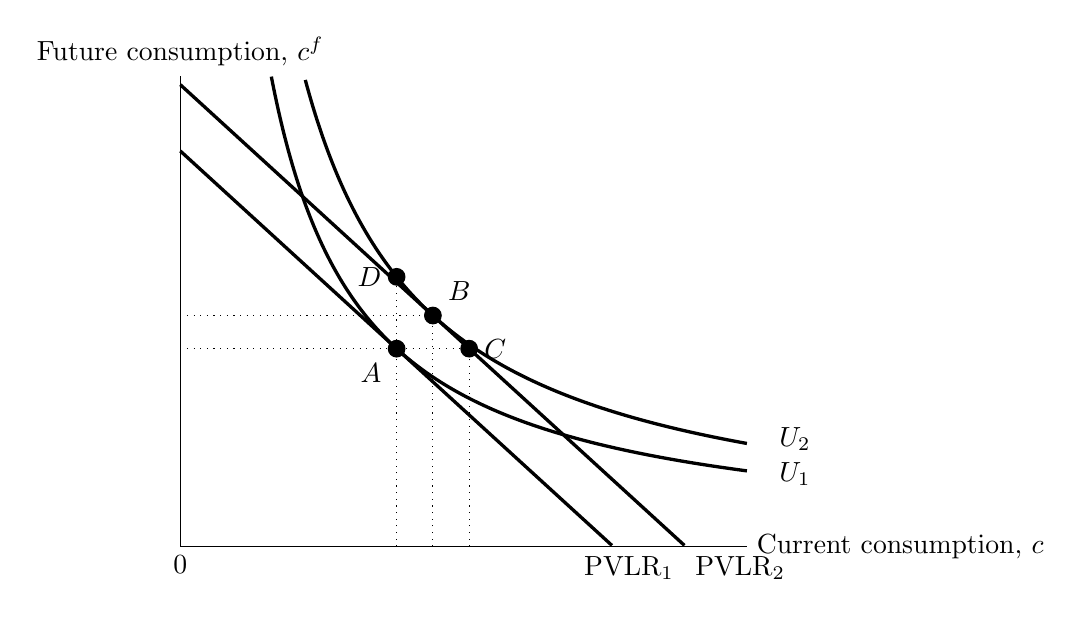
\begin{tikzpicture}
% ================== PARAMETERS (edit these) ==================
\pgfmathsetmacro{\r}{0.10}  % interest rate
\pgfmathsetmacro{\ay}{5.0}  % initial present resources (a+y)
\pgfmathsetmacro{\yf}{5.0}  % future endowment y^f
\pgfmathsetmacro{\aytwo}{\ay + 1.6} % shifted present resources (parallel shift)
% ============================================================

% ---- Derived quantities (do not edit) ----
\pgfmathsetmacro{\m}{-(1+\r)}                       % slope of both budgets
% A: tangency of initial budget with U1
\pgfmathsetmacro{\cA}{(\yf - \m*\ay)/(-2*\m)}
\pgfmathsetmacro{\cfA}{(1+\r)*\cA}
\pgfmathsetmacro{\kone}{(1+\r)*\cA*\cA}             % U1 level
% B: tangency of shifted budget with U2
\pgfmathsetmacro{\cB}{(\yf - \m*\aytwo)/(-2*\m)}
\pgfmathsetmacro{\cfB}{(1+\r)*\cB}
\pgfmathsetmacro{\ktwo}{(1+\r)*\cB*\cB}             % U2 level
% C: on shifted budget at same cf as A
\pgfmathsetmacro{\cfC}{\cfA}
\pgfmathsetmacro{\cC}{\aytwo + (\cfC-\yf)/\m}
% D: same c as A on the higher IC U2
\pgfmathsetmacro{\cfD}{\ktwo/\cA}
% PVLR intercepts
\pgfmathsetmacro{\PVLRone}{\ay + \yf/(1+\r)}
\pgfmathsetmacro{\PVLRtwo}{\aytwo + \yf/(1+\r)}

\begin{axis}[
  xmin=0, xmax=12.5,
  ymin=0, ymax=12.5,
  axis lines* = left,
  xtick={0}, ytick=\empty,
  clip=false,
  scale=1.05,
]

% ---------------- Budgets (solid black) ----------------
\addplot[domain=0:12.5, restrict y to domain=0:12.5, samples=400, color=black, very thick]
  {\yf + \m*(x-\ay)};     % Initial budget
\addplot[domain=0:12.5, restrict y to domain=0:12.5, samples=400, color=black, very thick]
  {\yf + \m*(x-\aytwo)};  % Shifted budget

% ---------------- Indifference curves ------------------
\addplot[domain=1:12.5, restrict y to domain=0:12.5, samples=400, color=black, very thick]
  {\kone/x};  % U1 through A (tangent to initial budget)
\addplot[domain=1:12.5, restrict y to domain=0:12.5, samples=400, color=black, very thick]
  {\ktwo/x};  % U2 through B (tangent to shifted budget)

% ---------------- Points -------------------------------
\addplot[color=black, mark=*, only marks, mark size=3pt] coordinates {(\cA,\cfA)};
\node[below left=2pt] at (\cA,\cfA) {$A$};

\addplot[color=black, mark=*, only marks, mark size=3pt] coordinates {(\cB,\cfB)};
\node[above right=2pt] at (\cB,\cfB) {$B$};

\addplot[color=black, mark=*, only marks, mark size=3pt] coordinates {(\cC,\cfC)};
\node[right=2pt] at (\cC,\cfC) {$C$};

\addplot[color=black, mark=*, only marks, mark size=3pt] coordinates {(\cA,\cfD)};
\node[left=2pt] at (\cA,\cfD) {$D$};

% ---------------- Guides (dotted) -----------------------
\addplot[color=black, dotted] coordinates {(\cA,0) (\cA,\cfD)};
\addplot[color=black, dotted] coordinates {(0,\cfA) (\cC,\cfA)};
\addplot[color=black, dotted] coordinates {(0,\cfB) (\cB,\cfB)};
\addplot[color=black, dotted] coordinates {(\cB,0) (\cB,\cfB)};
\addplot[color=black, dotted] coordinates {(\cC,0) (\cC,\cfC)};

% ---------------- Axis labels --------------------------
\node[right] at (current axis.right of origin) {Current consumption, $c$};
\node[above] at (current axis.above origin) {Future consumption, $c^{f}$};

% ---------------- Curve labels (well spaced) -----------
\node[right] at (13,\kone/13) {$U_1$};
\node[right, yshift=3pt] at (13,\ktwo/13) {$U_2$};

% ---------------- PVLR labels at x-intercepts ----------
\node[below right] at (\PVLRone-0.85,0) {$\mathrm{PVLR}_1$};
\node[below right] at (\PVLRtwo,0) {$\mathrm{PVLR}_2$};

\end{axis}
\end{tikzpicture}
\end{center}

Note that the following points represent
\begin{itemize}
    \item $A$: initial optimal consumption
    \item $B$: consumption smoothing, spending some and saving some
    \item $C$: spending it all
    \item $D$: saving it all
\end{itemize} 
\end{remarks}



\subsubsection{Riccardian Equivalence}
\begin{theorem}
    The \textbf{Riccardian Equivalence Proposition} states that tax cuts do not affect desired consumption or national saving because in the long run, because all government purchases must be paid for by taxes. 
\end{theorem}

\begin{remark}
    Empirically, tax cuts increases current consumption. Riccardian Equivalence is reconciled with empirical observations under assumptions of borrowing constraint. \\

    Suppose an individual faces borrowing constraints and cannot borrow. The individual  wants to spend up to $c^*$ but can only attain $c \leq a + y$. \\
    
    A one-time tax rebate can be seen as a relaxing of the borrowing contraints from $a + y$ up to some $a + \tilde{y}$.
    \begin{center}
    \includegraphics[width = 0.4\textwidth]{graphs/fig_4_6.jpg}
    \end{center}

    If 
    \begin{itemize}
        \item $a + \tilde{y} < c^*$ increase $c$ by the full amount of the tax rebate
        \item $a + \tilde{y} > c^*$ increase $c$ only up to $c^*$
    \end{itemize} 
\end{remark}

\begin{remarks}
    \textbf{Riccardian Assumptions}
    \begin{enumerate}
        \item Assuming REP does not hold 
        \begin{itemize}
            \item People spend some and save some, i.e. \textit{consumption smoothing}
            \[
            T \downarrow \implies c \uparrow, s \uparrow
            \]
        \end{itemize} 
        \item Assuming REP holds and \textbf{there are borrowing constraints}
        \begin{itemize}
            \item Borrowers facing constraints increase consumption, 
            \[
            T \downarrow \implies c \uparrow, s \downarrow
            \]
        \end{itemize}
        \item Assuming REP holds and there are no borrowing constraints 
        \[
        T \downarrow \implies c, s \text{ constant }
        \]
    \end{enumerate}
\end{remarks}

\subsubsection{Effects of an increase in interest rate}
\begin{definition}
    The \textbf{expected after-tax real interest rate} is the after-tax nominal interest rate minus expected rate of inflation 
    \[
        r_{a-t} = (1 - t)i - \pi^e
    \]
    Where 
    \begin{align*}
        i &= \text{ nominal interest rate} \\
        t &= \text{tax rate on interest income} \\
        pi^e &= \text{expected inflation}
    \end{align*}
\end{definition}
\begin{remarks}
    \textbf{Effect of an increase in interest rate on budget constraint}  
    \begin{itemize}
        \item $PVLR \downarrow$: present value of future income decreases
        \item vertical intecept $\uparrow$: future value of present income and assets increases 
        \item no-borrowing no-lending point remains the same 
        \item $c^*$: depends
    \end{itemize} 

    \begin{center}
    \includegraphics[width = 0.5\textwidth]{graphs/fig_4_1.jpg}
    \end{center}
\end{remarks}

\begin{remarks}
    \textbf{Effect of an increase in interest rate} \\

    \begin{minipage}{0.48\textwidth}
        \textbf{For borrowers}
        \begin{itemize}
            \item Substitution effect: $r \uparrow \implies s \uparrow c \downarrow$
            \item Income effect: $r \uparrow \implies s \uparrow c \downarrow$
        \end{itemize} 
    \begin{center}
    \includegraphics[width = 0.8\textwidth]{graphs/fig_4_2.jpg}
    \end{center}
    Borrowers \textbf{unequivocally consume less}.
    \end{minipage}
    \hfill
    \begin{minipage}{0.48\textwidth}
        \textbf{For lenders}
        \begin{itemize}
            \item Substitution effect: $r \uparrow \implies s \uparrow c \downarrow$
            \item Income effect: $r \uparrow \implies s \downarrow c \uparrow$
        \end{itemize} 
    \begin{center}
    \includegraphics[width = 0.8\textwidth]{graphs/fig_4_3.jpg}
    \end{center}
    Theory alone cannot predict the behavior of lenders when $r$ increases.
    \end{minipage}
\end{remarks}

\begin{remark}
    \textbf{Empirically}, an increase in interest rate causes a moderate decrease in consumption and a moderate increase in savings.
    \begin{center}
    \includegraphics[width = 0.4\textwidth]{graphs/fig_4_4.jpg}
    \end{center}
\end{remark}

\subsubsection{Effects of government purchases and taxes} 
Assumign no $NFP$ or $NX$, 
\begin{align*}
    S &= Y - C - G \\
    S_{priv} &= \underbrace{(Y - T)}_{\text{Disposable Income}} - C \\
    S_{govt} &= T - G
\end{align*}

\begin{remarks}
    \textbf{Effect of a tax cut}, assuming REP does not hold
    \begin{align*}
        \bar{Y} &= C + I + G \\
        T \downarrow & \implies ( \bar{Y} - T \downarrow ) \uparrow \implies C \uparrow \text{ by part} \\
        S &= \left( \bar{Y} - C \uparrow  - G \right)   \downarrow  \\
        \bar{Y}  &= C \uparrow \shortdownarrow + I \downarrow + G
    \end{align*}
\end{remarks}

\begin{remarks}
    \textbf{Effect of incrase in government purchases}
    \begin{align*}
        \bar{Y} &= C + I + G \uparrow \\
        S &= \left( \bar{Y} - C  - G \uparrow \right)   \downarrow  \\
        \bar{Y}  &= C \shortdownarrow \text{ a little }+ I \downarrow + G \uparrow
    \end{align*}
\end{remarks}


\subsubsection{Summary of factors affecting consumption}
\begin{remark}
    \textbf{Summary of factors affecting consumption}. \\
    \begin{center}
    \begin{tabular}{c | c | c}
    \textbf{Change} & $\Delta C$ & $\Delta S$ \\ \hline
    $y \uparrow$     & $c \uparrow$     & $s \uparrow$     \\
    $a \uparrow$     & $c \uparrow$     & $s \downarrow$   \\
    $y^{f} \uparrow$ & $c \uparrow$     & $s \downarrow$   \\
    $r \uparrow$     & $c \downarrow$   & $s \uparrow$     \\
    \end{tabular}
    \end{center}

\end{remark}

\subsection{Investment}

\begin{definition}
    A firm's \textbf{desired capital stock} is the profit-maximizing amount of capital for the firm.
\end{definition}

\begin{remark}
    The profit-maximizing level of capital is achieved when the expected future marginal benefit, \textit{expected future marignal product of capital}, $MPK^f$ is equal to the expected future marginal cost, \textit{user cost of capital}.
\end{remark}


\begin{definition}
    The \textbf{user cost of capital} is the expected real cost of a unit of capital for a specific period of time.  
    \[
        uc = (r + d) p_K
    \]
    Where
    \begin{align*}
        p_K &= \text{real price of capital goods} \\
        d &= \text{capital depreciation rate} \\
        r &= \text{expected real interest rate}
    \end{align*}
\end{definition}

\begin{remark}
    \textbf{Desired Capital Stock}
    \begin{center}
    \includegraphics[width = 0.5\textwidth]{graphs/fig_4_7.jpg}
    \end{center}
\end{remark}

\subsubsection{Changes in desired capital stock}
\begin{remark}
    \textbf{Effect of decrease in user cost of capital}

    \begin{center}
    \includegraphics[width = 0.5\textwidth]{graphs/fig_4_8.jpg}
    \end{center}
\end{remark}

\begin{remark}
    \textbf{Effect of an increase in marginal product of capital}
    \begin{center}
    \includegraphics[width = 0.5\textwidth]{graphs/fig_4_9.jpg}
    \end{center}
\end{remark}

\subsubsection{Effects of taxes on desired capital stock}
\begin{definition}
    The \textbf{tax-adjusted user cost of capital} is the user cost of capital divided by $1 + \tau$ where $\tau$ is the tax rate on firm revenues. \\
    \[
        \text{tax-adjusted user cost of capital} = 
        \frac{uc}{1 - \tau} = \frac{(r + d)p_K}{1 - \tau}
    \]
    

    Firms facing corporate taxes earn an after-tax future marginal product of capital 
    \[
    (1 - \tau) MPK^f
    \]

    Profit max capital stock occurs when 
    \[
        (1 - \tau) MPK^f = uc \implies MPK^f = \frac{uc}{1 - \tau} = \frac{(r + d)p_K}{1 - \tau}
    \]
\end{definition}

\subsubsection{Desired capital stock and investment}

\begin{definition}
    \textbf{Gross investment} is defined as the total purchase or construction of new capital goods. 
\end{definition}

\begin{definition}
    \textbf{Net investment} is defined as the difference between gross investment and depreciation.
    \[
    \underbrace{K_{t + 1} - K_t}_{\text{net investment}} = \underbrace{I_t}_{\text{gross investment}} - \underbrace{dK_t}_{ \text{ depreciation}}
    \]
    Where
    \begin{align*}
        I_t &= \text{gross investment in year $t$} \\
        K_t &= \text{capital stock in the beninging of year $t$} \\
        I_t &= \text{capital stock at the beninging of year $t + 1$} \\
    \end{align*}

    Assuming firms seek to match $K_{t + 1}$ to $K^*$,
    \[
        I_t = \underbrace{K^* - K_t}_{\text{desired net increase in capital stock}} + \underbrace{dK_t}_{\text{investment required to replace worn out capital}}
    \]
\end{definition}

\subsection{Goods Market Equilibrium}

\begin{definition}
    The \textbf{goods market equilibrium condition}, assuming a closed economy, states that the quantity of goods demanded is the sum of desired consumption, desired investment and government purchases 
    \[Y = C^d + I^d + G
    \]
\end{definition}

\begin{remark}
    The goods market equilibrium is \textbf{not the same} as the income-expenditure identity for a closed economy. \\

    The income-expenditure identity relates actual income to actual spending and is always satisfied. \\

    The goods market equilibrium condition may not always be satisfied. If firms produce more than consumers want to purchase
    \begin{itemize}
        \item inventory increases,
        \item income-expenditure identity remains true, increase in $Y$ matched by increase in $I$ (inventory spending) 
        \item goods-market equilibrium no longer holds, $Y > C^d + I^d + G$
    \end{itemize} 
\end{remark}

\begin{corollary}
    Goods market equilibrium implies that national saving is equal to desired investment. 
    \begin{align*}
        Y &= C^d + I^d + G \\
        Y - C^d - G &= I^d \\
        S^d &= I^d
    \end{align*}
\end{corollary}
\begin{center}
\includegraphics[width = 0.5\textwidth]{graphs/fig_4_10.jpg}
\end{center}

\subsubsection{Factors affecting savings curve}

\begin{remark}
    Savings decreases due to 
    \begin{itemize}
        \item decrease in current income
        \item increase in expected future income
        \item increase in wealth 
        \item increase in current taxes
        \item increase in government purchases
    \end{itemize} 
\end{remark}

\begin{center}
\includegraphics[width = 0.5\textwidth]{graphs/fig_4_11.jpg}
\end{center}


\begin{remark}
    \textbf{Effect of an adverse productivity shock} \\
    An adverse productivity shocks lowers labor demand and qunatity of labor 
    \[A \downarrow \implies NS \downarrow \overline{N} \downarrow
    \]

    Also, an adverse productivity shock lowers output 
    \[
    A \downarrow \implies A\downarrow F( K, N) = Y\downarrow
    \]

    Since $S = Y - C - G$, and $\bar{Y} \downarrow$, the decrease in income lowers $C$ and $S$ by part via consumption smoothing.

\end{remark}

\begin{remark}
    \textbf{Effect of an increase in wealth} \\

    Given an increase in wealth, individuals consume more due to consumption smoothing. 
    \[
        C \uparrow \implies S = (Y - C \uparrow - G) \downarrow
    \]
\end{remark}


\begin{remark}
    Summary of factors affecting goods-market equilibrium  \\

    \begin{center}
    \begin{tabular}{l l c c}
    	\textbf{Change} & \textbf{Description} & $\Delta C$ & $\Delta S$ \\\hline
    $A \downarrow$ & Total factor productivity & $\downarrow$ & $\downarrow$ \\
    $G \uparrow$ & Government purchases & $\shortdownarrow$ a little & $\downarrow$ \\
    Wealth $\uparrow$ & Increase in household wealth & $\uparrow$ & $\downarrow$ \\
    $T \downarrow$ & Taxes on households & $\uparrow$ followed by  $\shortdownarrow$ a little & $\uparrow$ \\
    $\tau \downarrow$ & Business (corporate) tax rate & $\shortdownarrow$ a little & $\shortuparrow$ a little \\
    \end{tabular}
    \end{center}
\end{remark}



